\documentclass[10pt,conference,compsocconf]{IEEEtran}

\usepackage[hidelinks]{hyperref}
\usepackage{graphicx}
\usepackage{booktabs}
\usepackage{amsmath}

\begin{document}
\title{Predicting Coronary Heart Disease from BRFSS Survey Answers\\with Linear Models}

\author{
  Author One, Author Two, Author Three\\
  \textit{CS-433 Machine Learning, EPFL, Switzerland}
}

\maketitle

\begin{abstract}
We predict whether a respondent of the 2015 Behavioral Risk Factor
Surveillance System (BRFSS) survey reports coronary heart disease or a heart
attack (MICHD), using only linear models implemented in NumPy. Only 8.8\% of
respondents are positive, so we optimize the F1 score of the positive class.
The main gains come from encoding the survey correctly rather than from the
model: treating ``don't know''/``refused'' codes as missing and one-hot
encoding categorical answers with missingness as its own level raise the
cross-validated F1 of logistic regression from 0.411 to 0.435. Our final model
reaches F1 0.438 on an untouched holdout and 0.448 on the AIcrowd test set.
\end{abstract}

\section{Introduction}

The dataset contains 328,135 labeled and 109,379 unlabeled respondents, each
described by 321 survey variables (demographics, health status, behaviors,
preventive care). The label is $+1$ if the respondent reports having been told
they had coronary heart disease, angina or a heart attack. Two properties shape
the problem: the classes are imbalanced (a constant negative predictor reaches
91.2\% accuracy and F1 = 0), and the features are survey answers whose numeric
codes are not quantities (e.g.\ \texttt{GENHLTH}=9 means ``refused'', not
``worse health than 5''). We report F1 of the positive class as the main
metric, as on the competition leaderboard, together with accuracy and the
threshold-free ROC AUC.

\section{Models and Methods}

\subsection{Data preprocessing}
\label{sec:preprocessing}
All preprocessing parameters are learned on training rows only and stored for
reuse on validation and test rows. Starting from the baseline below, we
evaluate each step separately (Table~\ref{tab:ablation}).

\textbf{Baseline.} Every column is used as a number. Interview metadata and
identifiers (date, sequence number, sampling unit, state) and columns with more
than 50\% missing values are dropped; missing values are imputed with the
median; features are standardized (163 features).

\textbf{Clean codes.} BRFSS encodes non-answers inside the value range, with a
width that depends on the question~\cite{brfss15}: 7/9 for one-digit answers
(7 only when the scale stops before 6, e.g.\ \texttt{EMPLOY1}=7 is
``retired''), 77/99, 777/999 and 7777/9999 for wider ones. These become
missing values. Codes 88/888 mean ``none'' in day counts (e.g.\ days of poor
physical health) and become 0. Ten columns where these rules are wrong were
checked against the codebook and overridden (e.g.\ in height in inches, 77 is
a real height). We also drop survey design weights and 14 raw columns with
mixed units or frequency formats (weight, height, drinks, fruit, exercise),
for which the dataset already contains cleaned derived versions.

\textbf{One-hot encoding.} Columns with at most 10 distinct valid values (211
of 321) are one-hot encoded, with missing as an additional level, the most
frequent level as reference, and levels rarer than 0.1\% merged into it.
Keeping missingness as a level matters because values are missing by design:
follow-up questions are only asked when relevant. For example, the age at
diabetes diagnosis is missing for non-diabetics; the positive rate is 22.1\%
when it is observed and 6.9\% when it is not. All columns are therefore kept,
whatever their missing rate.

\textbf{Full.} The 73 continuous columns are additionally clipped to their
0.5--99.5\% training percentiles, standardized on observed rows only, filled
with 0 when missing, and given a binary missing indicator. Constant and
duplicate columns are removed, giving 637 features plus a bias term.

\subsection{Models}
We implemented the six required methods: linear regression by gradient descent
(GD) and stochastic GD, least squares and ridge regression through the normal
equations, and logistic regression with and without an $L_2$ penalty
$\lambda\|w\|^2$ by GD. Least squares and ridge are trained on $\{0,1\}$ labels
and their outputs are thresholded directly. Logistic regression uses the
numerically stable loss $\frac{1}{N}\sum_n \log(1+e^{x_n^\top w}) - y_n
x_n^\top w$, step size $\gamma=0.5$ and 500 full-batch steps from $w=0$. This
is converged for every feature set: 2,000 steps change the training loss by
less than $10^{-4}$, while $\gamma=2$ settles at a higher loss.

\subsection{Evaluation protocol}
We hold out a stratified 20\% of the labeled rows (65,627) and use them once,
to score the final model. On the remaining 80\% we run 5-fold stratified
cross-validation with preprocessing refitted inside every fold. Folds are
identical across experiments, so we report the paired fold-wise difference
$\Delta$F1 between consecutive configurations. Because of the class imbalance,
the decision threshold on $\sigma(x^\top w)$ is a hyperparameter: we choose the
F1-maximizing value on the pooled out-of-fold scores and report the mean $\pm$
standard deviation of F1 over folds at that threshold.

\section{Results}

\begin{table}[tbp]
  \centering
  \caption{Cross-validated ablation of the preprocessing (5 folds, 262,508
  rows). Logistic regression, $\lambda=0$. $\Delta$F1: paired difference to
  the previous row.}
  \label{tab:ablation}
  \begin{tabular}{@{}lccccc@{}}
    \toprule
    Preprocessing & $D$ & F1 & $\Delta$F1 & AUC & Ridge F1 \\
    \midrule
    Baseline     & 163 & .411$\pm$.004 & --            & .849 & .406 \\
    Clean codes  & 143 & .424$\pm$.004 & +.013$\pm$.002 & .858 & .415 \\
    One-hot      & 578 & .435$\pm$.006 & +.011$\pm$.004 & .863 & .425 \\
    Full         & 637 & .436$\pm$.005 & +.000$\pm$.001 & .863 & .426 \\
    \bottomrule
  \end{tabular}
\end{table}

\textbf{Preprocessing.} Cleaning the codes and one-hot encoding each improve F1
by more than 0.01 in every fold (Table~\ref{tab:ablation}), and AUC rises with
them, so the gain is not a threshold effect. Missing indicators and clipping
bring no measurable change once missingness is one-hot encoded. Logistic
regression outperforms ridge regression by about 0.01 F1 for every feature set.

\textbf{Regularization.} On the full features, the CV F1 of logistic regression
is flat for $\lambda \in \{0, 10^{-6}, \dots, 10^{-3}\}$ (0.4351--0.4356) and
decreases at $\lambda=10^{-2}$ (0.4327). With 262k rows for 637 features the
model does not overfit; we keep $\lambda=10^{-4}$, the best mean.

\begin{figure}[tbp]
  \centering
  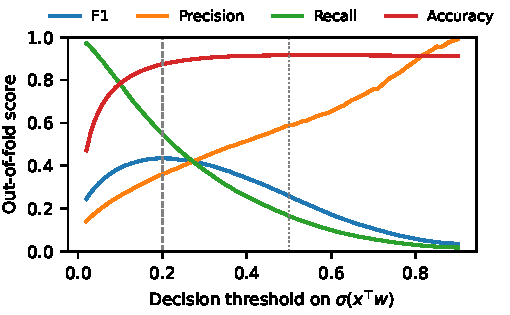
\includegraphics[width=\columnwidth]{figures/threshold}
  \caption{Out-of-fold metrics of the final model against the decision
  threshold. Dashed: selected threshold 0.20; dotted: 0.5.}
  \label{fig:threshold}
\end{figure}

\textbf{Threshold.} At the default threshold 0.5 the final model has the
highest accuracy (0.916) but finds only 16.6\% of positives (F1 0.259).
Lowering the threshold to 0.20 trades accuracy (0.874) for recall (0.549) and
maximizes F1 at 0.436 (Fig.~\ref{fig:threshold}). Precision stays low (0.36):
most respondents flagged as at risk do not report MICHD.

\begin{table}[tbp]
  \centering
  \caption{Final evaluation. Holdout: 65,627 rows never used for selection.}
  \label{tab:final}
  \begin{tabular}{@{}lcccc@{}}
    \toprule
    Model (threshold) & F1 & Prec. & Recall & AUC \\
    \midrule
    All negative          & 0     & --   & 0    & .500 \\
    Baseline logistic (0.20)  & .417 & .340 & .539 & .851 \\
    Full, $\lambda=10^{-4}$ (0.20) & \textbf{.438} & .363 & .554 & .866 \\
    \midrule
    AIcrowd test: baseline / final & \multicolumn{4}{l}{.411 / \textbf{.448}} \\
    \bottomrule
  \end{tabular}
\end{table}

\textbf{Final model.} Refitted on the 80\% and scored once, the selected model
reaches F1 0.438 on the holdout (Table~\ref{tab:final}), in line with its
cross-validated F1 of 0.436. Refitted on all labeled rows, it scores 0.448 on
the AIcrowd test set, against 0.411 for the baseline.

\section{Discussion}
Both preprocessing gains come from respecting how the survey was answered,
not from adding model capacity: special codes carry no magnitude, and the
pattern of skipped questions is itself informative. Once these are encoded,
regularization, missing indicators and the number of GD steps have no
measurable effect, which suggests that the linear model, not the amount of
data, now limits performance. Interaction features or non-linear models are
the natural next steps.

The labels are self-reported past diagnoses, so the model detects respondents
who \emph{already} report MICHD from answers that may be consequences of the
disease (e.g.\ medication or general health); it does not estimate the risk
of developing it, and its coefficients are not causal. F1 also depends on the
8.8\% prevalence and would change on a population with a different one.

\section{Summary}
Encoding BRFSS answers as categories, with special codes and skipped questions
as information, improves F1 from 0.411 to 0.436 in cross-validation, and the
final regularized logistic regression reaches 0.438 on a holdout and 0.448 on
the test set. All results are reproduced by the scripts in our repository
(\texttt{model\_selection.py}, \texttt{run.py}).

\bibliographystyle{IEEEtran}
\bibliography{literature}

\end{document}
